\documentclass[a4j,8pt,twocolumn]{extarticle}

% ---------------

\usepackage{winf-paper}
\usepackage{amsmath}
\usepackage{amssymb}
\usepackage{ascmac}
\usepackage{latexsym}
\usepackage{ulem}
\usepackage{url}
\usepackage[dvipdfmx]{graphicx}

% ---------------

%% 和文題目
\title{声に対する印象を用いた合成音声ライブラリ探索サービスの提案}

%% 和文著者
\author{情報 太郎 \qquad 情報 花子}

%% 和文所属
\affiliation{情報大学情報学部}





% ===== 所属が複数の場合 =====
%\author{情報 太郎\DAG{1} \qquad 情報 花子\DAG{1} \qquad 情報 次郎\DAG{2}}
%\affiliation{\DAG{1}情報大学情報学部 \qquad \DAG{2}情報大学大学院情報学研究科}
%\eauthor{Taro Info\DAG{1} \qquad Hanako Info\DAG{1} \qquad Jiro Info\DAG{2}}
%\eaffiliation{%
%	\DAG{1} Faculty of Information, Information University\\
%	\DAG{2} Graduate School of Information, Information University
%}

\begin{document}

\maketitle
\thispagestyle{empty}	% 1ページ目のページ番号を表示しない
% ------------------------------------------------------------

\section{はじめに}

人の歌声や喋り声を人工的に再現する音声合成ソフトは数多く存在しており,それらソフトのほとんどが複数種類の声を切り替えて使用できる.
また,その中でもいくつかのソフトでは個人が声の元となる合成音声ライブラリを作成し,第三者による利用を前提とした配布を行える.
例えば,喋り声を対象とした合成音声ソフトCOEIROINKではユーザの作成した音声合成モデルが350キャラクタ分以上配布されているほか\cite{mycoeiroink},歌声を対象とした合成音声ソフトUTAUでは同ソフト上で使用できるUTAU音源ライブラリが7000キャラクタ分以上存在する\cite{vdbutau}.
このように,今や合成音声ソフトの利用者は使える声に対し非常に多くの選択肢を持っており,その全ての把握は現実的ではない.

合成音声を利用するシーンにおいて,声が持つイメージや印象は声を選ぶ上で考慮すべき要素である.
例えば喋らせるアナウンスの内容や,歌わせる曲調など用途に合った声質を持つライブラリを選択し,用いるのは制作において重要なプロセスである.
しかし,現状声の持つ印象を知るには実際に聴いてみるのが最も有力な手段であり,数多あるライブラリの生み出す声を十分な数聴き比べ適切な声を採択するには多大な手間と時間を要する.
その結果として,ユーザがライブラリを選ぶ際,その多くが普段の生活の中で聞いた経験のある声や,知っているキャラクターの声を選択していると考えられる.
これはユーザ全体の中で使われる声に大きな偏りを生じさせてしまう.
万に近い数存在するライブラリのうち実際にユーザに用いられる声は一握りであり,ほとんどのライブラリはユーザに用いられず埋もれてしまう.

\begin{figure}[h]
  \centering
  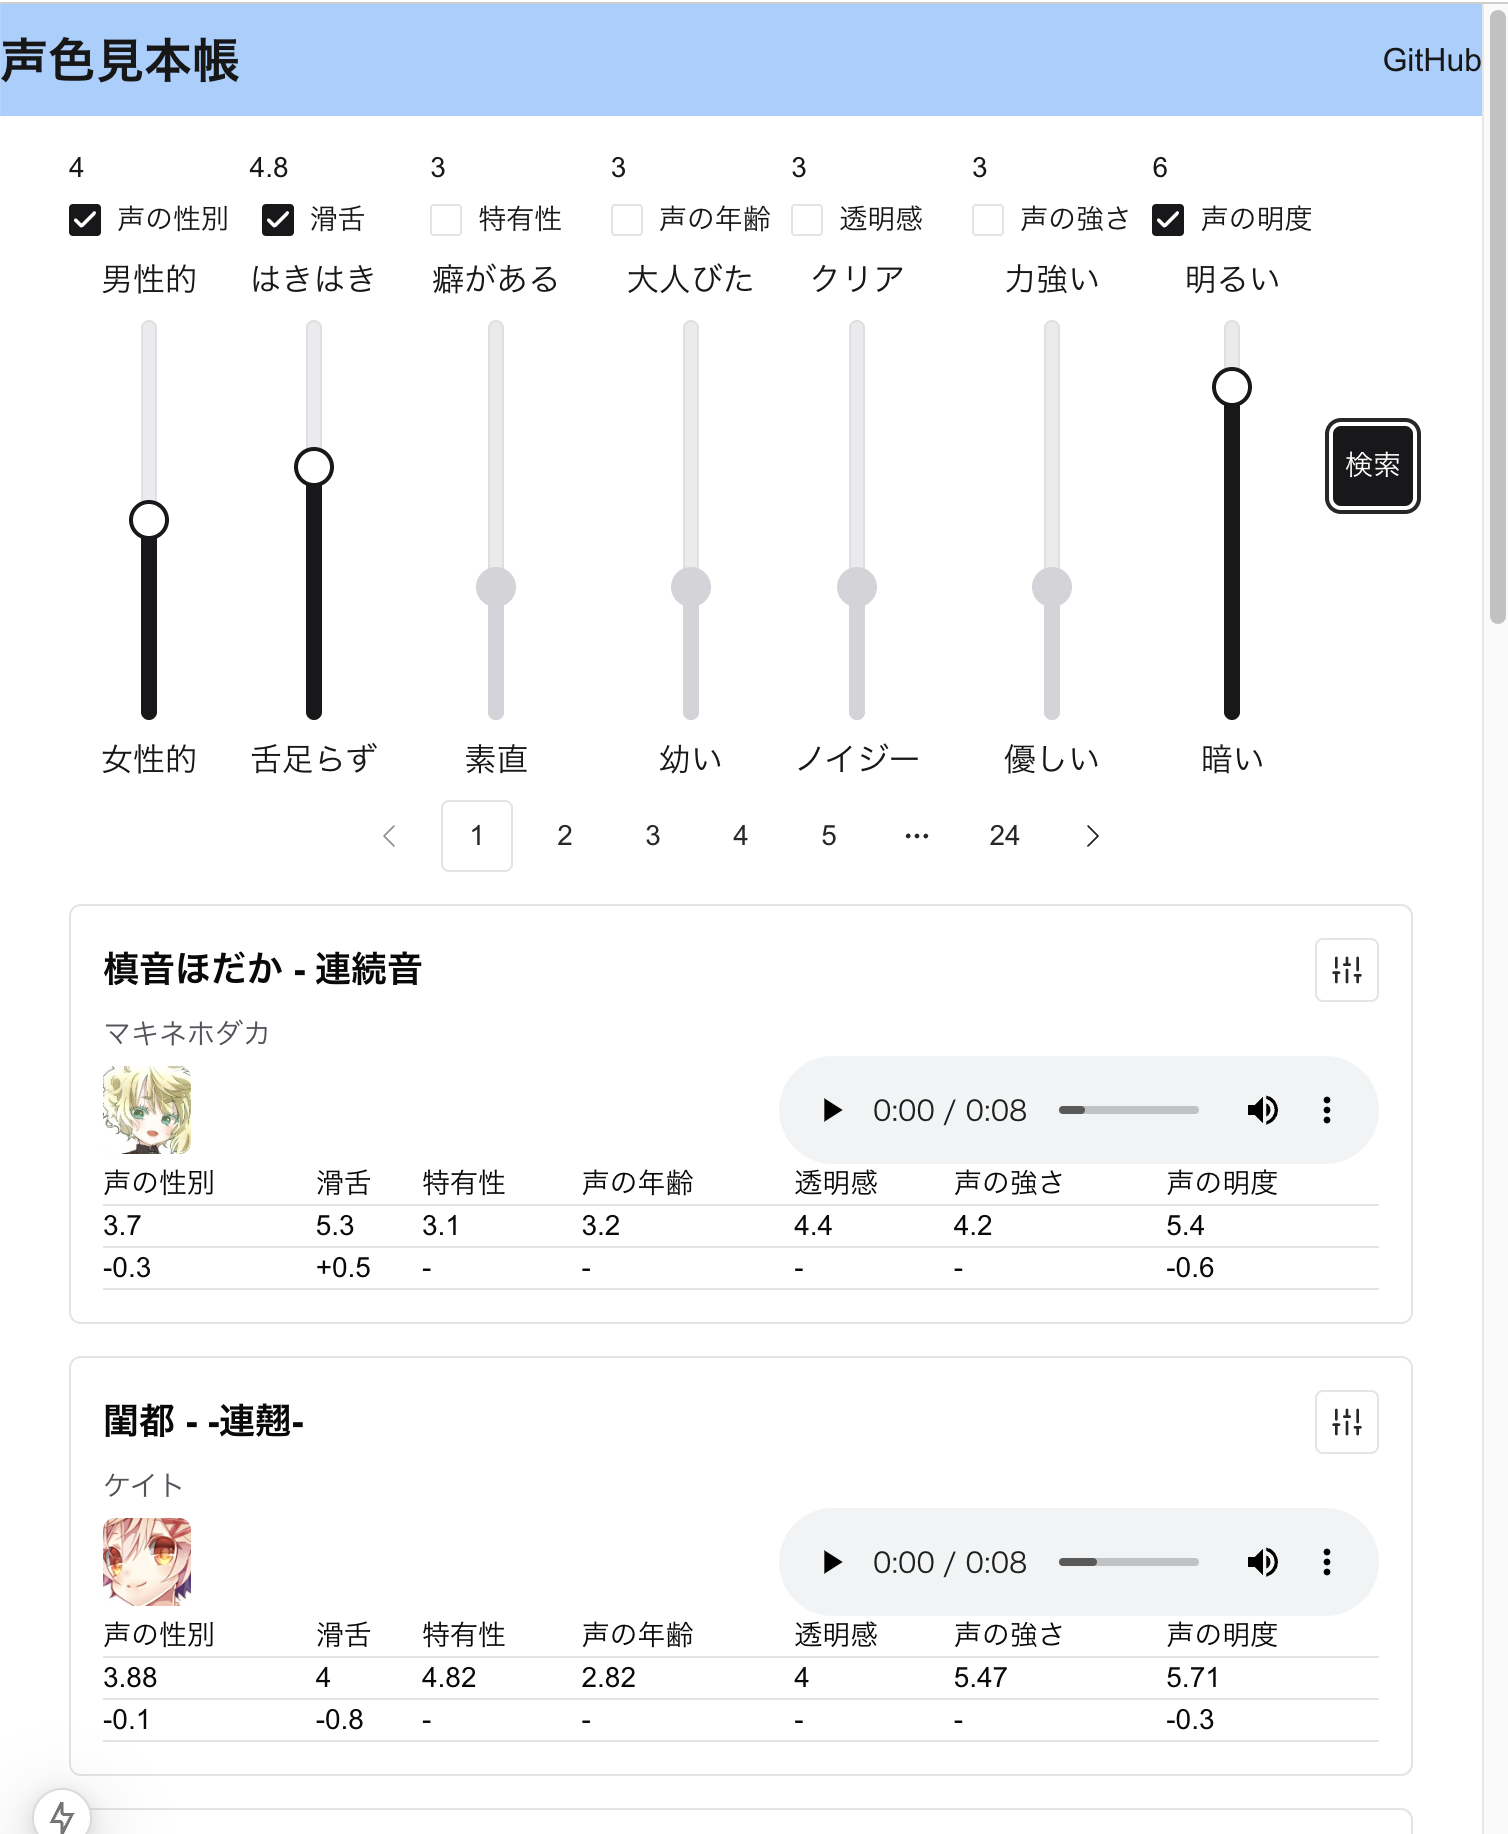
\includegraphics[width=0.9\linewidth]{fig/site_image.png}
  \caption{システムの画面イメージ}
  \label{fig:site_image}
\end{figure}

そこで本研究では,ライブラリごとの声に対する印象を事前に数値化し,それを用いてユーザの求める声に近いライブラリを探索するシステムを提案する.
探索対象とする合成音声ソフトは特に利用できるライブラリが多く,後述する声質に関するアンケートが存在しているUTAU音源ライブラリを対象とする.
本システムでは事前に,声に対する印象を複数の印象軸ごとに評価スコアとして数値化する.
ユーザは理想としてイメージする声の評価スコアを入力し,目的に合った音源を探索できる.
評価スコアの軸には,例えばスコアの高低を女性らしい声・男性らしい声に対応させた"性別感"など,ユーザが声からスコアを,あるいはスコアから声をある程度想定できるような直感的な軸が望ましい.
各音源に対する評価スコアは,アンケート調査によって集められたデータをもとに音源ファイルから各評価スコアを推定できる機械学習モデルを作成し,それを用いて付与する.
また,本システムは多くの人が手軽に利用できるようWebアプリケーションとして実装する.

% ------------------------------------------------------------
\section{関連研究}
\subsection{アマチュア歌唱者に向けた歌声可視化方法の検討}
本研究に関連する研究として,人間の歌声から印象やイメージされる色を推定する研究\cite{ama}がある.
この研究では,ある程度の長さがある歌声と,そのうちの瞬間的な長さの歌声を用い,それぞれで印象を推定するモデルを作成している.
ある程度の長さがある歌声では,迫力性,丁寧さ,明るさの3軸に対してそれぞれのスコアを推定するモデルを作成し,推定を行なった.
結果として,人の間でも印象の評価が大きく揺れるような歌唱などの例外を除き,十分な精度で印象を推定できた.
また歌声のうち瞬間的な音声からは印象に加え,声に対してイメージされる色を推定する試みも行っている.
彩度など色の要素と表現語の一つとして挙げられた活動性との関係が見られるなど,声質の色での表現に対して一定の有効性が示されたものの,他の要素との関係については今後の課題とされている.
この研究から,声質へのなんらかの評価軸を用いた評価スコア付与が可能である点や,それを用いた声質の表現は一つの手段として妥当なものであると考えられる.

\subsection{声質にスコアを付与する研究}
UTAU音源を対象に声質に対し評価スコアを付与し,そのスコアを用いて音源を探索するシステムを提案する研究\cite{ong}が存在する.
この研究でも本研究と同じくUTAUに評価スコアを付与,探索システムを構築し,実際にユーザが求める声を探索できるかを確認している.
スコアの推定にはUTAUを用いて合成された音声データを用い,重回帰分析とカーネル回帰分析での推定制度の比較を行なっている.
また,推定されたスコアを用いて音源を探索する際には,ある2つのスコア行列間のユークリッド距離を目標類似距離とし,その逆数として定義した目標類似度を用いて音源を探索している.
評価実験では,ユーザのイメージする声に近いスコアを入力し,目標類似度の高いライブラリを提示した.するとユーザが求めるような声を持つライブラリを探索できる結果が示された.
一方でこの研究では,探索システムの実装に留まっており,探索アルゴリズムの検討や実際にユーザが利用するシステムの提案は行われていない.

\subsection{可視化・探索するシステムを提供するサービス}
クリプトン・フューチャー・メディア株式会社と産業総合研究所によって開発された音楽発掘サービス「Kiite(キイテ)」では、その機能の一つとして「Kiite Radar」が提供されている\cite{kiite}.
ユーザは,楽曲の知名度やニコニコ動画上でのマイリスト率,楽曲を歌っているキャラクターなどの一般的な楽曲情報での絞り込みに限らず,楽曲の解析によって得られた曲の声質や踊りたくなるかどうかの印象をスライダーで設定し,その条件に合致する楽曲を探索するできる.
加えて,全ての楽曲を分析した印象に基づいて2次元平面上にプロットされた印象マップが提供されている.
激しい曲は左上に,軽快な曲は右上にプロットされるなど楽曲の配置には一定の傾向があり,ユーザはこれらを用いて直感的に楽曲を探索できる.
対象が歌声でなく楽曲である点は異なるが,本来数値ではない印象を数値化し,それを用いて可視化・探索するという点で本研究と共通する部分があり,サービスを提供する上で参考にできる.

% ------------------------------------------------------------
\section{*声質に対する評価スコアの推定}
本研究では,UTAU音源ライブラリに対して声質に対する評価スコアを付与するための機械学習モデルを作成する.
それぞれのライブラリの音声から抽出した特徴量と,事前にアンケート調査などによって得られた評価スコアを用い,特徴量から評価スコアを推定するモデルを作成する.
評価スコアの推論には学習データとしてUTAU音源声質アンケートのデータを,モデル作成にはPythonライブラリであるPyCaretを用いた.

\subsection{特徴量の抽出}
特徴量を抽出するためには,ライブラリを用いて複数の音階で「あ」「い」「う」「え」「お」「ん」と発声した音声ファイルを利用する.
五母音と子音「ん」は連続して発声のできる音素であり,安定して音声の特徴を抽出できる.
音階はA3,D4,G4,C5,F5の5音階を用いる.
複数の音階を用いる特徴量の数を増加させるほか,音声の音域による特徴への影響などを反映できると考えられる.

実際に用いる特徴量としては,MFCC,ZCR,F1〜F4の周波数を採用した.
MFCCとは,音声の周波数成分を人間の聴覚特性に基づいて変換したものであり,音声の特徴を抽出するために広く用いられる.
MFCCのうち高次元の成分は話者認識に用いられるなど,音声の声質に関連するとされる\cite{}ため,本研究ではMFCCを64次元まで取得し用いる.
ZCRは音声の振動数を表す指標であり,音の高さやノイズの大きさによって振動数は変化する.
音声の声高を固定した今回の音声であれば,音声の声質に関連する指標として扱えると考え採用した.
音響フォルマントは音声の共振周波数を表す指標であり,母音の識別に用いられる.
同じ音素のフォルマント周波数でも話者の年齢や性別によって変化があり\cite{formant},声の印象に影響があると考えられる.
本研究では各音階と音素ごとのF1〜F4の周波数を取得し用いる.

\subsection{モデルの構築}
モデルの構築にはPythonライブラリであるPyCaretを用いた.
PyCaretは機械学習モデルの作成を簡略化するためのライブラリであり,データの前処理からモデルの選定,評価までを一連の流れで行える.
UTAU音源声質アンケートの結果はExcelファイルとして提供されている.
このファイルに記載されている240種のUTAU音源ライブラリのうち,現在でもダウンロードが可能であり,必要な音素が収録されていて,かつ利用規約上で研究目的を含む機械学習用途での利用が禁止されていない168ライブラリを対象とした.
各評価スコアを推論の目標として与え,先述の特徴量から評価スコアを推定するモデルを評価スコアの7軸それぞれについて別々に作成した.
学習時には,使用するライブラリから3割をランダムに選びテストデータとして,残りのデータを学習データとして用いた.
学習モデルはPyCaretで選択できる多数の手法の中から,それぞれの評価スコアに対して各手法で初期モデルを作成し,最も推論に適していると思われる手法を主にR2値から判断して選定し,学習を行った.

\subsection{UTAU音源ライブラリとUTAU音源声質アンケート}
本研究において探索対象とするUTAU音源ライブラリは,無償で公開されている歌唱用音声合成ソフトであるUTAU上で使用できる音源ファイルであり,ソフトと同じく無償で公開されているものが多い.
UTAUは波形接続と呼ばれる手法を用いており,音声データを切り貼りして音声を合成する.
そのため,UTAU音源ライブラリは主に合成に用いるためにできる限り一定の音程と音量になるように収録された収録者の肉声が収録されている.
収録形式には複数の手法があり,単独音であれば各wavファイルにひらがな1文字に対応する音素が収録されており,連続音(VCV)であれば「あんああいあうあ」\cite{tatsu3shiki}といった形で複数の音素が連続して収録されている.

本研究で実際に特徴量を抽出する際,音声合成は行わずこのwavファイルを直接操作し音声合成の手間を削減した.
必要な音素が収録された音声ファイルのうち,UTAUにおいては子音部とブランクとして指定されるタイミング間の音声を利用した.
この範囲はUTAU上で音声が合成される際母音を伸ばすために用いる範囲であり,一般に安定して同じ声が収録されているため音声の特徴を抽出する上で適していると考えられる.
複数音階の音声の生成には,音階ごとにライブラリで指定されるwavファイルからピッチシフトを行い,音声を生成した.

UTAU音源声質アンケートはニコニコ大百科上で提言されたUTAU音源ライブラリに対する声の特徴を評価するためのアンケート規格であり,現在までにこの規格を用いて250種以上のUTAU音源ライブラリに対してアンケートが行われている.
このアンケートは表\ref{tab:survey}に示す7項目について,それぞれ1から7までの7段階評価で10件以上のアンケート調査を行い,その平均を評価値としている.
アンケートは各UTAU音源ライブラリごとに行われ,表情音源が複数存在する場合は各表情音源ごとに独立してアンケートが行われている.

\begin{table}[htb]
  \centering
  \caption{UTAU音源声質アンケートの評価軸}
  \label{tab:survey}
  \begin{tabular}{c|cc}
    \hline
    評価軸 & 低い値の示す表現語 & 高い値の示す表現語 \\
    \hline
    声の性別 & 女性的 & 男性的 \\
    滑舌 & 舌足らず & はきはき \\
    特有性 & 素直 & 癖がある \\
    声の年齢 & 幼い & 大人びた \\
    透明感 & ノイジー & クリア \\
    声の強さ & 優しい & 力強い \\
    声の明度 & 暗い & 明るい \\
    \hline
  \end{tabular}
\end{table}

UTAU音源ライブラリは数が多い点だけでなく,声質の依存先が生の音声ファイルである点や,音素情報を関連づけるiniファイルが一般的に用いられる形式であるため非常に扱いやすい点,UTAU音源声質アンケートが存在する点が評価できる.
無償で利用できるものがほとんどである点も,多くの合成音声の中から用いたい声を探したい利用者のニーズに合っている.
ライブラリの声質を評価する上で,また利用者からの目線においても都合が良いと考え,本研究の対象として選定した.

\subsection{*結果の評価}
構築したモデルによる推論の精度を評価するため,テストデータに対して推論を行い得た値と実際のアンケートによって得られた値を比較した.
テストデータは先述の通り学習データからランダムに選ばれたデータであり,対象とした168ライブラリの3割にあたる51ライブラリを用いた.
7つの評価軸それぞれについて,テストデータでの精度を評価した結果を図\ref{tab:score_coor},図\ref{tab:score_box}に示す.

\begin{figure}[h]
  \centering
  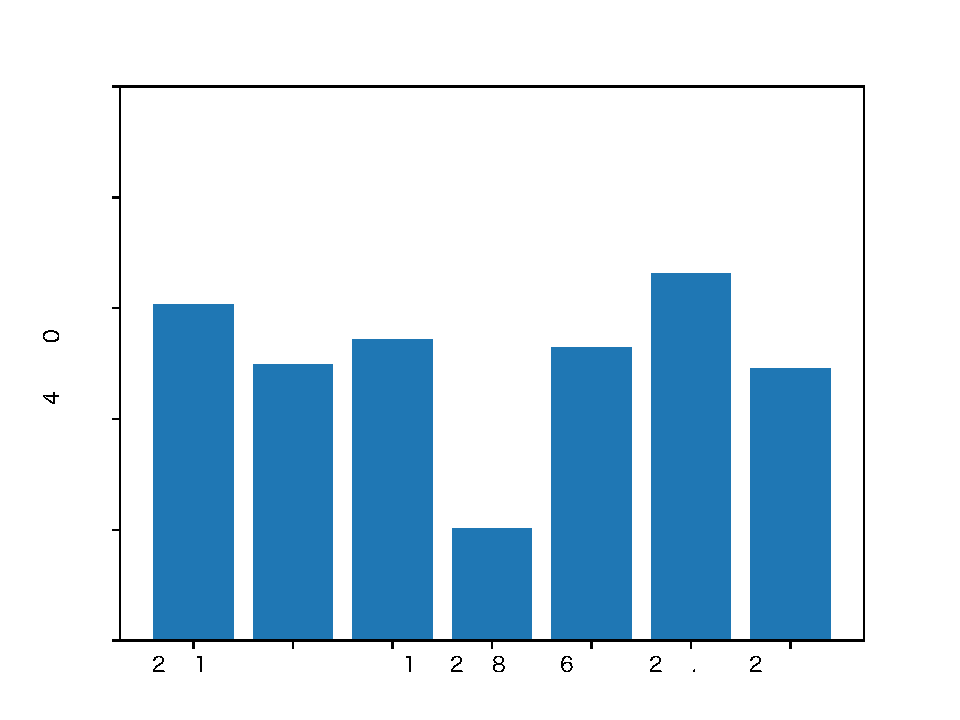
\includegraphics[width=\linewidth]{fig/model_quality_coor.pdf}
  \caption{テストデータとの相関係数}
  \label{tab:score_coor}
\end{figure}

\begin{figure}[h]
  \centering
  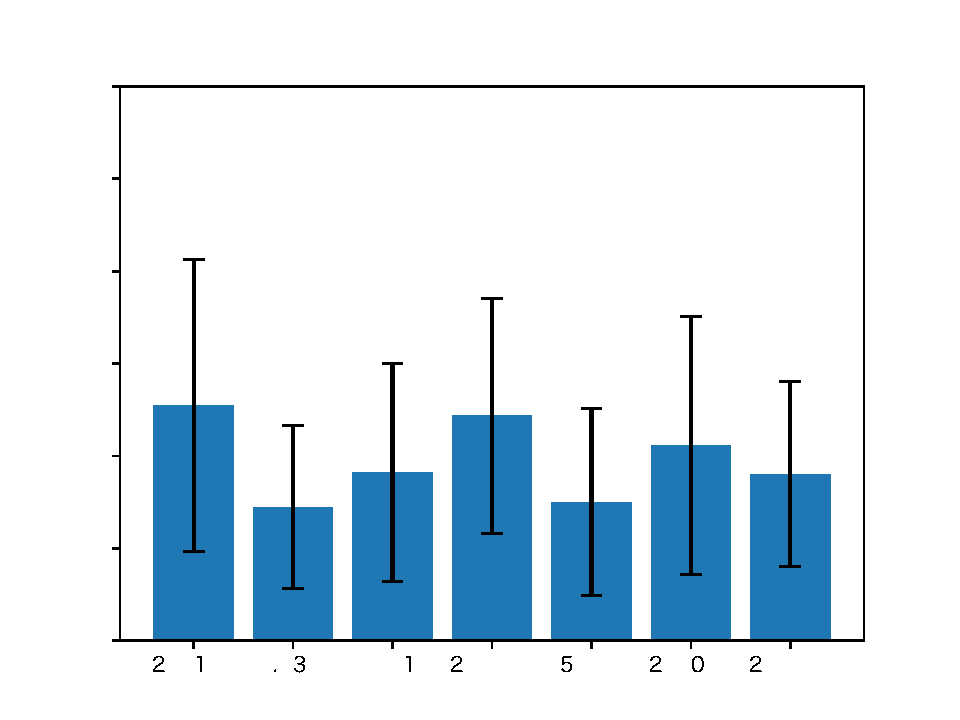
\includegraphics[width=\linewidth]{fig/model_quality_rms.pdf}
  \caption{テストデータとの誤差の二乗平均平方根}
  \label{tab:score_box}
\end{figure}

図\ref{tab:score_coor}では,横軸は評価軸を,縦軸はテストデータにおける実際の値と推測された値との相関係数を示している.
相関係数は一般に0.7以上であればデータ間に強い相関が,0.4以上であればある程度の相関があるとされ,実際の値と推測された値における相関が強いほど推論の精度が高いと言える.
結果を見ると,最も低い声の年齢では0.2,他の評価軸では0.5から0.6程度となっており,推論の精度は高くはないものの一定の相関が見られた.

図\ref{tab:score_box}では,横軸は評価軸を,縦軸はテストデータにおける実際の値と推測された値との誤差の二乗平均平方根(RMS),エラーバーは誤差の標準偏差を示している.
RMSは実際の値と推測された値の誤差を示す指標であり,誤差が小さいほど推論の精度が高いと言える.
結果として誤差のRMSは最も高い声の性別で1.3となった.
これは先行研究\cite{dnn}の精度に近く,先行研究にて示された音響特徴量を用いたモデルの精度が再現できたと言える.

% ------------------------------------------------------------
\section{声色見本帳}
\subsection{システムの概要}
本研究で提案するシステム「声色見本帳」は,ユーザが求める声の評価スコアを入力し,その評価スコアに近い合成音声ライブラリを探索・提案するシステムである.
このサービスを利用すると,ユーザは自身が求める声に近いライブラリを探すことができ,多くのライブラリの中から自身に合った声を見つけることができる.
システムはWebアプリケーションとして実装し,ユーザはブラウザ上で利用できる.
システムの画面イメージを図\ref{fig:screen}に示す.

\subsubsection{ライブラリ探索}
ユーザは求める声の評価スコアを入力し,その評価スコアに近いUTAU音源ライブラリを探索できる.
ユーザは先に述べた7項目のうち、任意の数の評価軸に対してスライダーを操作し,評価スコアを入力する.
システムは入力された評価スコアに近いライブラリを探索し,その結果をユーザに提示する.
評価スコアの近さは,ユーザに選択された評価軸での平方ユークリッド距離によって判断し,距離の昇順にライブラリを並べる.

\subsubsection{ライブラリ詳細の表示}
ユーザが探索結果として提示されたライブラリを選択すると,そのライブラリの詳細情報を表示する.
詳細情報にはライブラリの名前,推定された評価スコア,サンプル音声,ライブラリの公式サイトや配布ページへのURLなどが含まれる.
サンプル音声としては,童謡の「かえるのうた」をPythonライブラリ「ScoreDraft」を用い事前に生成したファイルを用いる.
本サービスはユーザが求める声に近いライブラリの探索のみを目的としているため,直接ライブラリをダウンロードする機能は提供せず,ユーザが自身でURL先からダウンロードするよう促す.
また,選択したライブラリの評価スコアを検索欄に転写できる.
この機能を用いれば,あるライブラリに近い声質のライブラリを探したり,探索結果ページを送り反対に遠い声質のライブラリを探せる.

\subsubsection{探索対象ライブラリの追加}
ユーザはUTAU音源ライブラリをアップロードし,サイト上に存在しないUTAUライブラリを自由に追加できる.
すでに構築されたモデルを用いて評価スコアやサンプル音声などを自動で生成し,システムに追加する.
ユーザがライブラリを追加できるため,より多くのライブラリや,この先新しく生まれ配布されるライブラリに対してもシステムを適用できる.

\subsection{*システムの評価}
\begin{enumerate}
  \item システムを実際に使ってもらい,ユーザが求める声に近いライブラリを探索できるかを評価する.
  \item また,システムの使いやすさや機能の拡張性についても評価する.
\end{enumerate}

% ------------------------------------------------------------
\section{おわりに}

% ------------------------------------------------------------
\begin{thebibliography}{9}
\bibitem{mycoeiroink}
COEIROINC,
MYCOEIROINK.
\url{https://coeiroink.com/mycoeiroink/list}

\bibitem{vdbutau}
Vocaloid Database.
\url{https://vocadb.net/Search?searchType=Artist&artistType=UTAU}

\bibitem{ama}
金礪愛,
アマチュア歌唱者に向けた歌声可視化方法の検討.
博士論文,早稲田大学,2018

\bibitem{ong}
山根壮一ほか,
歌声合成システムの音源データに対する声質推定と声質制御.
情報処理学会研究報告,Vol.2015-MUS-108,No.6,pp.1-6,2015

\bibitem{dnn}
横森文哉,大柴まりや,森勢将雅,小澤賢司,
スペクトル包絡情報を入力としたDeep Neural Networkに基づく歌声のための声質評価
情報処理学会音楽情報科学研究会,Vol.2015-MUS-107,No.61,1-6,2015

\bibitem{zcr}
佐賀 圭真,井村 誠孝,
発話音声の聞き取りやすさ向上のための音声特徴量解析.
エンタテインメントコンピューティングシンポジウム2019論文集,2019,pp.84-86,2019

\bibitem{formant}
粕谷英樹ほか,
年令, 性別による日本語5母音のピッチ周波数とホルマント周波数の変化,
日本音響学会誌,24巻,6号,pp.355-364,1968

\bibitem{kiite}
産業総合研究所,
音楽印象分析・音楽推薦を駆使して楽曲と出会える音楽発掘サービス「Kiite」を公開
\url{https://www.aist.go.jp/aist_j/press_release/pr2019/pr20190830/pr20190830.html}

\bibitem{tatsu3shiki}
巽式 連続音の録音リスト配布 - 巽のブログ,
\url{https://tatsu3.hateblo.jp/entry/ar426004}

\bibitem{utausurvey}
ニコニコ大百科,
UTAU音源声質アンケートとは,
\url{https://dic.nicovideo.jp/a/utau%E9%9F%B3%E6%BA%90%E5%A3%B0%E8%B3%AA%E3%82%A2%E3%83%B3%E3%82%B1%E3%83%BC%E3%83%88}
% \url{https://dic.nicovideo.jp/a/utau音源声質アンケート}

\end{thebibliography}


% ------------------------------------------------------------
\end{document}
